\chapter{Ensembles of cost-sensitive decision trees}\label{ch:9}

\begin{remark}{Outline}
In this chapter, we introduce the framework of ensembles of example-dependent cost-sensitive 
decision-trees, by training example-dependent cost-sensitive decision trees using four different 
random inducer methods and then blending them using three different combination approaches.
First, in Section \ref{sec:9:ensemble}, we give the background behind ensemble learning. Then, in 
Section \ref{sec:9:ecsdt}, we present our previously proposed ensembles of cost-sensitive 
decision-trees framework. Moreover, in Section \ref{sec:9:theoretical}, we prove theoretically that 
combining individual cost-sensitive classifiers achieves better  results in the sense of higher 
financial savings. Finally, in Section \ref{sec:9:experiments}, we compare the results of the 
proposed algorithm, against state-of-the-art methods, using the five real-world cost-sensitive 
databases.
\end{remark}

\section{Ensemble methods}
\label{sec:9:ensemble}

Ensemble learning is a widely studied topic in the machine learning community. The main idea behind 
the ensemble methodology is to combine several individual base classifiers in   order to have a 
classifier that outperforms each of them \citep{Rokach2009}. Nowadays,   ensemble methods are  one 
of the most popular and well studied machine learning techniques   \citep{Zhou2012}, and it can be 
noted that since 2009 all the first-place and   second-place winners of the KDD-Cup 
competition\footnote{\url{https://www.sigkdd.org/kddcup/}}   used  ensemble methods. The core 
principle in ensemble learning, is to induce random perturbations into  the learning procedure in 
order to produce several different base classifiers from a single  training set, then combining the 
base classifiers in order to make the final prediction.  In order to induce the random permutations 
and therefore create the different base classifiers,   several methods have been proposed, in 
particular: bagging \citep{Breiman1996},   pasting~\citep{Breiman1999}, random forests 
\citep{Breiman2001} and random patches   \citep{Louppe2012}. Finally, after  the base   classifiers 
are trained, they are typically   combined using either   majority voting,  weighted  voting    or  
stacking~\citep{Zhou2012}.

\begin{figure}[t!]
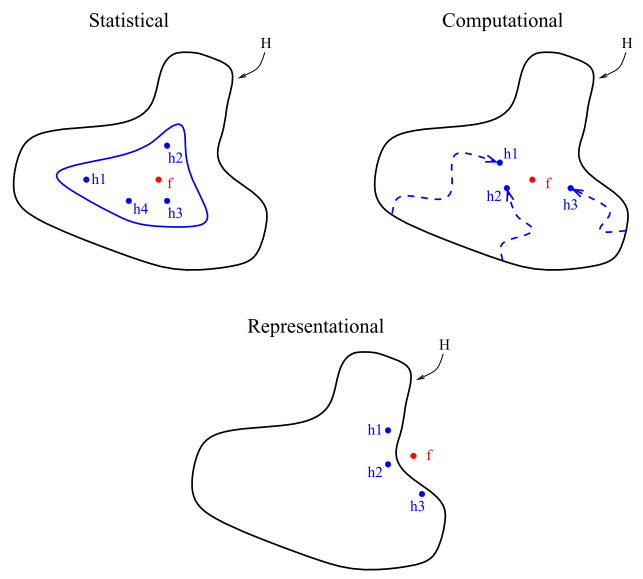
\includegraphics[scale=.4]{ch9_fig1}
\caption{Main reasons regarding why ensemble methods perform better than 
  single models: statistical, computational and representational \citep{Dietterich2000a}.}
\label{fig:9:1}
\end{figure} 

As shown in \figurename{~\ref{fig:9:1}, there are three main reasons regarding why ensemble 
methods perform better than single models: statistical, computational and representational 
\citep{Dietterich2000a}. First, from a statistical point of view, when the learning set is too 
small, an algorithm can find several good models within the search space, that arise to the same 
performance on the training set $\mathcal{S}$. Nevertheless, without a validation set, there is 
a risk of choosing the wrong model. The second reason is computational; in general, algorithms 
rely on some local search optimization and may get stuck in a local optima. Then, an ensemble may 
solve this by focusing different algorithms to different spaces across the training set. The last 
reason is representational. In most cases, for a learning set of finite size, the  true function 
$f$ cannot be represented by any of the candidate models. By combining several  models in an 
ensemble, it may be possible to obtain a model with a larger coverage across the  space of 
representable functions.
  

  
  The most typical form of an ensemble is made by combining $T$ different base classifiers.
  Each  base classifier $M(\mathcal{S}_j)$ is trained by applying algorithm $M$ to a random subset 
  $\mathcal{S}_j$ of the training set $\mathcal{S}$.  %  $\mathcal{S_j} = RI(\mathcal{S})$
  For simplicity we define $M_j \equiv  M(\mathcal{S}_j)$ for $j=1,\dots,T$, and 
  $\mathcal{M}=\{M_j\}_{j=1}^{T}$ a set of base classifiers.
  Then, these models are combined using majority voting to create the ensemble $H$ as follows
  \begin{align}\label{eq:9:majority-vote}
    f_{mv}(\mathcal{S},\mathcal{M}) = \argmax_{c \in \{0,1\}} \sum_{j=1}^T 
    \mathbf{1}_c(M_j(\mathcal{S})).
  \end{align}


  \begin{remark}{Theoretical performance of an ensemble}
%   Moreover, i
  If we assume that each one of the $T$ base classifiers has a probability $\rho$ of 
  being correct, the probability of an ensemble making the correct decision, denoted by $P_c$,
  can be calculated using the binomial \mbox{distribution \citep{Hansen1990}}
  \begin{equation}\label{eq:9:prob}
    P_c = \sum_{j>T/2}^{T} {{T}\choose{j}} \rho^j(1-\rho)^{T-j}.
  \end{equation}
  Furthermore, as shown in \cite{Lam1997}, if $T\ge3$ then:
  \begin{equation}\label{eq:9:Pc}
  \lim_{T \to  \infty} P_c= \begin{cases} 
            1  &\mbox{if } \rho>0.5 \\ 
            0  &\mbox{if } \rho<0.5 \\ 
            0.5  &\mbox{if } \rho=0.5 ,
            \end{cases}
  \end{equation}
	leading to the conclusion that 
	\begin{equation}\label{eq:9:Pc2}
  \rho \ge 0.5 \quad \text{and} \quad T\ge3 \quad \Rightarrow \quad P_c\ge \rho.
  \end{equation}
  \end{remark}
  
\subsection{Cost-sensitive ensembles}

  In the context of cost-sensitive classification, some authors have proposed methods for using 
  ensemble techniques. In \citep{Masnadi-shirazi2011}, the authors proposed a framework for 
  cost-sensitive boosting that is expected to minimized the losses by using optimal cost-sensitive 
  decision rules. In \citep{Street2008}, a bagging algorithm with adaptive costs was proposed. In 
  his doctoral thesis, Nesbitt \citep{Nesbitt2010}, proposed a method for cost-sensitive 
  tree-stacking. In this method different decision trees are learned, and then combined in a way 
  that a cost function is minimize. Lastly in \citep{Lomax2013}, a survey of application of 
  cost-sensitive learning with decision trees is shown, in particular including other methods that 
  create cost-sensitive ensembles. However, in all these methods, the  misclassification costs only 
  dependent on the class, therefore, assuming a constant cost across  examples. As a consequence, 
  these methods are not  well suited for example-dependent cost-sensitive  problems. 

      
\section{Ensembles of cost-sensitive decision trees}
\label{sec:9:ecsdt}

In this section we shown our previously proposed framework of ensembles of  example-dependent 
cost-sensitive  decision-trees \citep{CorreaBahnsen2015b}, by training example-dependent 
cost-sensitive decision trees using four different  random inducer methods and then blending them 
using three different combination approaches. Moreover, we propose two new cost-sensitive 
combination approaches, cost-sensitive weighted  voting and cost-sensitive stacking. The latter 
being an extension of our previously proposed cost-sensitive logistic regression 
\citep{CorreaBahnsen2014b}. 

The remainder of the section is organized as follows: First, we introduce the different random 
inducers used to create the base classifiers. Then, we present the combination methods. Finally, we 
define our proposed algorithms.


\subsection{Random inducers}

With the objective of creating an ensemble of example-dependent cost-sensitive decision trees, we 
first create $T$ different random subsamples $\mathcal{S}_j$ for $j=1,\dots,T$, of the training  
set 
$\mathcal{S}$, and train a $CSDT$ algorithm on each one. In particular we create the different 
subsets using four different methods: bagging \citep{Breiman1996}, pasting \citep{Breiman1999}, 
random forests \citep{Breiman2001} and random patches \citep{Louppe2012}. 

In bagging \citep{Breiman1996}, base classifiers are built on randomly drawn bootstrap subsets of 
the original data, hence producing different base classifiers. Similarly, in pasting 
\citep{Breiman1999}, the base classifiers are built on random  samples without replacement from 
the training set. In random forests \citep{Breiman2001}, using decision trees as the base learner, 
bagging   is extended and   combined  with a  randomization of the input features that  are used 
when  considering candidates  to split    internal nodes. In particular, instead of looking for  
the best  split among all   features, the   algorithm selects, at each node, a random subset of 
features  and then determines   the best split only over  these features. In the random patches   
algorithm \citep{Louppe2012}, base classifiers are created by randomly     drawn bootstrap subsets 
of both examples and features. To further clarify the difference between the random inducer 
methods, in \figurename{~\ref{fig:9:2}}, we show a visual representation of the random inducers 
algorithms.
 
\begin{figure}[t!]
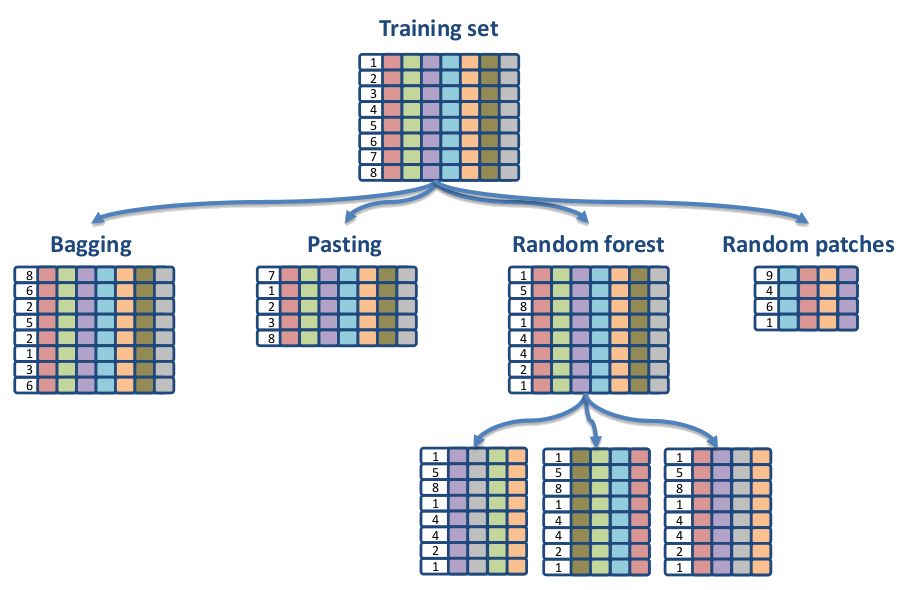
\includegraphics[scale=.5]{ch9_fig2}
\caption{Visual representation of the random inducers algorithms.}
\label{fig:9:2}
\end{figure} 


\subsection{Combination methods}

Lastly, the base classifiers are combined using either majority voting, cost-sensitive weighted 
voting and cost-sensitive stacking. Majority voting consists in collecting the predictions of 
each base classifier and selecting the decision with the highest number of votes, see 
(\ref{eq:9:majority-vote}).

\subsubsection{Cost-sensitive weighted voting}

This method is an extension of weighted voting. First, in the traditional approach, a 
similar comparison of the votes of the base classifiers is made, but giving a weight $\alpha_j$ 
to each classifier $M_j$ during the voting phase \citep{Zhou2012}
\begin{align} \label{eq:9:weighted-majority-vote}
  f_{wv}(\mathcal{S},\mathcal{M}, \alpha)
  =\argmax_{c \in \{0,1\}} \sum_{j=1}^T \alpha_j \mathbf{1}_c(M_j(\mathcal{S})),
\end{align}
where $\alpha=\{\alpha_j\}_{j=1}^T$.
The calculation of $\alpha_j$ is related to the performance of each classifier $M_j$.
It is usually defined as the normalized misclassification error   $\epsilon$ of the base 
classifier $M_j$  in the out of bag set   $\mathcal{S}_j^{oob}=\mathcal{S}-\mathcal{S}_j$
\begin{equation}
  \alpha_j=\frac{1-\epsilon(M_j(\mathcal{S}_j^{oob}))}{\sum_{j_1=1}^T 
  1-\epsilon(M_{j_1}(\mathcal{S}_{j_1}^{oob}))}.
\end{equation}

\noindent However, as previously discussed, the misclassification measure is not suitable in  many 
real-world classification problems. We  herein propose a method to calculate the weights $\alpha_j$ 
 taking into account the actual savings of the classifiers. Therefore using (\ref{eq:3:savings}), we 
define
\begin{equation}
  \alpha_j=\frac{Savings(M_j(\mathcal{S}_j^{oob}))}
  {\sum_{j_1=1}^T Savings(M_{j_1}(\mathcal{S}_j^{oob}))}.
\end{equation}
This method guaranties that the base classifiers that contribute to a higher increase in savings 
have more importance in the ensemble.

\subsubsection{Cost-sensitive stacking}
\label{sec:9:staking}

The staking method consists in combining the different base classifiers by learning a 
second level algorithm on top of them \citep{Wolpert1992}. In this framework, once the base 
classifiers are constructed using the training set  $\mathcal{S}$, a new set is constructed 
where the output of the base classifiers  are now considered as the features while keeping the 
class labels.

Even though there is no restriction on which algorithm can be used as a second level learner, 
it is common to use a linear model \citep{Zhou2012}, such as 
\begin{align}
  f_s(\mathcal{S},\mathcal{M},\beta) =
  g \left( \sum_{j=1}^T \beta_j M_j(\mathcal{S}) \right),
\end{align}
where $\beta=\{\beta_j\}_{j=1}^T$, and $g(\cdot)$ is the sign function 
\mbox{$g(z)=sign(z)$} in the case of a linear regression or the sigmoid function, defined 
as \mbox{$g(z)=1/(1+e^{-z})$}, in the case of a logistic regression. 

Moreover, following the logic used in \citep{Nesbitt2010}, we propose learning the set of  
parameters $\beta$  using our proposed cost-sensitive logistic regression ($CSLR$) 
\citep{CorreaBahnsen2014b}. The $CSLR$ algorithm consists in introducing example-dependent costs 
into a logistic regression, by changing the objective function of the model to one that is 
cost-sensitive. For the specific case of cost-sensitive stacking, we define the cost function as: 
\begin{align}
  &J(\mathcal{S},\mathcal{M},\beta)= 
  \sum_{i=1}^{N} \bigg[ y_i\bigg( 
  f_s(\mathbf{x}_i,\mathcal{M},\beta) \cdot(C_{TP_i} - C_{FN_i}) + C_{FN_i} \bigg) 
  \nonumber \\
  & + (1-y_i)\bigg( f_s(\mathbf{x}_i,\mathcal{M},\beta) \cdot(C_{FP_i} - C_{TN_i}) 
    +C_{TN_i} \bigg) \bigg].
\end{align}
Then, the parameters $\beta$ that minimize the logistic cost function are used in order to 
combine the different base classifiers. However, as discussed in \citep{CorreaBahnsen2014b}, 
this cost function is not convex for all possible cost matrices, therefore, we use genetic 
algorithms to minimize it.

Similarly to cost-sensitive weighting, this method guarantees that the base classifiers that 
contribute to a higher increase in savings have more importance in the ensemble. Furthermore, 
by learning an additional second level cost-sensitive method, the combination is made such that 
the overall   savings measure is maximized.


\subsection{Algorithms}

Finally, Algorithm \ref{alg:9:algorithms} summarizes the $ECSDT$ methods. In total, we   
evaluate 12 different algorithms, as four different random inducers (bagging, pasting, random 
forest and random patches) and three different combinators (majority voting, cost-sensitive 
weighted voting and cost-sensitive stacking) can be selected in order to construct the 
cost-sensitive ensemble.
  

\begin{algorithm}\label{alg:9:algorithms}
The proposed $ECSDT$ algorithms.
\textnormal{
\begin{algorithmic}[1]
\Require $CSDT$ (an example-dependent cost-sensitive decision tree algorithm), $T$ the number of 
iterations, $\mathcal{S}$ the training set, $inducer$, $N_e$ number of 
examples for each base classifier, $N_f$ number of examples for each base classifier, 
$combinator$.
\Function{ECSDT}{$\mathcal{S},T,inducer,N_e,N_f,combinator$}
  \State \textbf{Step 1:} Create the set of base classifiers
  \For{$j  \leftarrow 1$ to $T$}
    \State \textbf{switch}($inducer$)
    \State \textbf{case} Bagging:
      \State $\mathcal{S}_j \leftarrow $ Sample $N_e$ examples from $\mathcal{S}$ with replacement.
    \State \textbf{case} Pasting:
      \State $\mathcal{S}_j \leftarrow $ Sample $N_e$ examples from $\mathcal{S}$ without
      replacement.
    \State \textbf{case} Random forests:
      \State $\mathcal{S}_j \leftarrow $ Sample $N_e$ examples from $\mathcal{S}$ with replacement.
    \State \textbf{case} Random patches:
      \State $\mathcal{S}_j \leftarrow $ Sample $N_e$ examples and $N_f$ features from  
      $\mathcal{S}$ with replacement.
    \State \textbf{end switch}
    \State $M_j \leftarrow CSDT(\mathcal{S}_j)$
    \State $\mathcal{S}_j^{oob} \leftarrow \mathcal{S}-\mathcal{S}_j$
    \State $\alpha_j \leftarrow Savings( M_j(\mathcal{S}_j^{oob}))$
  \EndFor
  \State \textbf{Step 2:} Combine the different base classifiers
  \State \textbf{switch}($combinator$)
  \State \textbf{case} Majority voting:
  \State  $H \leftarrow f_{mv}(\mathcal{S}, \mathcal{M})$
  \State \textbf{case} Cost-sensitive weighted voting:
  \State $H \leftarrow f_{wv}(\mathcal{S}, \mathcal{M}, \alpha)$
  \State \textbf{case} Cost-sensitive stacking:
  \State $\beta \leftarrow \argmin_{\beta \in \mathbb{R}^T} 
        J(\mathcal{S},\mathcal{M},\beta)$
  \State  $H \leftarrow f_{s}(\mathcal{S}, \mathcal{M},\beta)$
  \State \textbf{end switch}
  \State \Return $H$
\EndFunction
\end{algorithmic}
}
\end{algorithm}
 
\section{Theoretical analysis of the ECSDT}
\label{sec:9:theoretical}

  Although the above proposed algorithm is simple, there is %little 
  no work that has formally 
  investigated ensemble performance in terms other than accuracy. In this section, our aim is to 
  prove theoretically that combining individual cost-sensitive classifiers achieves better results 
  in the sense of higher savings.
  
  We denote $\mathcal{S}_a$ $a\in \{0,1\}$, as the subset of $\mathcal{S}$ 
  where the examples belong to the class $a$:
  \begin{equation}\label{eq:9:S_a}
    \mathcal{S}_a = \{\mathbf{x}_i^* \vert y_i = a, i \in 1,\dots,N\},
  \end{equation}
  where $\mathcal{S}=\mathcal{S}_0 \cup \mathcal{S}_1$, $\mathcal{S}_0 \cap \mathcal{S}_1 = 
  \varnothing$, and $N_a=\vert \mathcal{S}_a \vert$. Also, we define the average cost of the base 
  classifiers as:
  \begin{align}\label{eq:9:avg_cost}
    \overline{Cost} (\mathcal{M}(\mathcal{S}))= \frac{1}{T} \sum_{j=1}^{T} Cost(M_j(\mathcal{S})). 
  \end{align}
  
  \noindent Firstly, we prove the following lemma that states the cost of an ensemble $H$ on the 
  subset $\mathcal{S}_a$ is lower than the average cost of the base classifiers on the same set for 
  $a  \in \{0,1\}$.

  \begin{lemma}\label{lemma1}
  Let $H$ be an ensemble of $T\ge3$ classifiers $\mathcal{M}=\{M_1, M_2,\dots,M_T\}$, and 
  $\mathcal{S}$ a testing set of size $N$. If each one of the base classifiers has a probability 
  of being correct higher or equal than one half, $\rho \ge \frac{1}{2}$, and the 
  \textit{reasonableness conditions} of the cost matrix are satisfied, then the following holds true
  \begin{align}\label{eq:9:lemma}
    Cost(H(\mathcal{S}_a)) &\le \overline{Cost} (\mathcal{M}(\mathcal{S}_a)) , \quad a  \in\{0,1\},  
 \end{align}
  \end{lemma}
  
  \noindent\begin{proof}
  First, we decompose the total cost of the ensemble by applying equations (\ref{eq:3:cost_total}) 
  and (\ref{eq:3:cost}). Additionally, we separate the analysis for $a=0$ and $a=1$:

  \textbullet\ $a=0:$
  \begin{align}
  Cost(H(\mathcal{S}_0)) =& \sum_{i=1}^{N_0} y_i(c_i C_{TP_i} + (1-c_i)C_{FN_i})+ \nonumber \\  
    & (1-y_i)(c_i C_{FP_i} + (1-c_i)C_{TN_i}) . 
  \end{align}
  
  \noindent Moreover, we know from (\ref{eq:9:prob}) that the probability of an ensemble 
  making the right decision, i.e., $y_i=c_i$, for any given  example, is equal to $P_c$. 
  Therefore, we can use this probability to estimate the expected savings of an ensemble: 
  \begin{align}\label{eq:21}
    Cost(H(\mathcal{S}_0)) &= \sum_{i=1}^{N_0} P_c C_{TN_i} +(1-P_c)C_{FP_i}.
  \end{align}
  
  \textbullet\ $a=1:$
  
  \noindent In the case of $\mathcal{S}_1$, and following the same logic as when $a=0$, the cost of 
  an  ensemble is:
  \begin{align}\label{eq:22}
    Cost(H(\mathcal{S}_1)) &= \sum_{i=1}^{N_1} P_c C_{TP_i} + (1-P_c)C_{FN_i}.  
  \end{align}

  \noindent The second part of the proof consists in analyzing the right hand side of 
  (\ref{eq:9:lemma}),   specifically, the average cost of the base classifiers on set 
  $\mathcal{S}_a$. To do that, with the help of (\ref{eq:3:cost_total}) and (\ref{eq:9:avg_cost}), 
  we may express the average cost of the base classifiers as:
  \begin{align}
    \overline{Cost} (\mathcal{M}(\mathcal{S}_a)) = \frac{1}{T} \sum_{j=1}^{T} \sum_{i=1}^{N_a} 
    Cost(M_j(\mathbf{x}_i^*)).  
  \end{align} 
  
  \noindent We define the set of base classifiers that make a negative prediction as
  \begin{align}
    \mathcal{T}_{i0}=\{M_j(\mathbf{x}_i^*) \vert M_j(\mathbf{x}_i^*) = 0, j \in 1,\dots,T\},
  \end{align}
  similarly, the set of classifiers that make a positive prediction as
  \begin{align}
    \mathcal{T}_{i1}=\{M_j(\mathbf{x}_i^*) \vert M_j(\mathbf{x}_i^*) = 1, j \in 1,\dots,T\}.
  \end{align}
  Then, by taking the cost of negative and positive predictions from (\ref{eq:3:f_a}), the 
  average cost of the base learners becomes:
  \begin{align}
    \overline{Cost} (\mathcal{M}(\mathcal{S}_a)) =& 
    \frac{1}{T} \sum_{i=1}^{N_a} \bigg( \vert \mathcal{T}_{i0} \vert \cdot 
    Cost(f_0(\mathbf{x}_i^*)) \nonumber \\
    & + \vert \mathcal{T}_{i1} \vert \cdot Cost(f_1(\mathbf{x}_i^*)) \bigg).
  \end{align} 

  \noindent We separate the analysis for $a=0$ and $a=1$:
  
  \textbullet\ $a=0:$
  
  \begin{align}
    \overline{Cost} (\mathcal{M}(\mathcal{S}_0)) =& \sum_{i=1}^{N_0} \bigg( 
    \frac{\vert \mathcal{T}_{i0} \vert}{T} \cdot C_{TN_i}
    + \frac{\vert \mathcal{T}_{i1} \vert}{T} \cdot C_{FP_i}\bigg).
  \end{align}
  Furthermore, we know from (\ref{eq:9:prob}) that an average base classifier will have a correct 
  classification probability of $\rho$, then $\frac{\vert \mathcal{T}_{i0} \vert}{T}=\rho$, leading 
  to:
  \begin{align}\label{eq:26}
    \overline{Cost} (\mathcal{M}(\mathcal{S}_0)) =& \sum_{i=1}^{N_0}  
    \rho \cdot C_{TN_i} + (1-\rho) \cdot C_{FP_i} .
  \end{align}

  \textbullet\ $a=1:$
 
 \noindent Similarly, for the set $\mathcal{S}_1$, the average classifier will have a correct 
  classification probability of $\rho$, then $\frac{\vert \mathcal{T}_{i1} \vert}{T}=\rho$. 
  
  \noindent Therefore,
  \begin{align}\label{eq:27}
    \overline{Cost} (\mathcal{M}(\mathcal{S}_1)) =& \sum_{i=1}^{N_1}  
    \rho \cdot C_{TP_i} + (1-\rho) \cdot C_{FN_i} .
  \end{align}
 
	\noindent Finally, by replacing in (\ref{eq:9:lemma}) the expected savings of an  ensemble with 
  (\ref{eq:21}) for $a=0$ and (\ref{eq:22}) for $a=1$, and the average cost of the base learners 
  with  (\ref{eq:26}) for $a=0$ and (\ref{eq:27}) for $a=1$, (\ref{eq:9:lemma}) is rewritten as:
  
  \noindent for $a=0$:
  \begin{align}\label{eq:9:lemma1}
    \sum_{i=1}^{N_0} P_c C_{TN_i} +(1-P_c)C_{FP_i} \le 
    \sum_{i=1}^{N_0} \rho \cdot C_{TN_i} + (1-\rho) \cdot C_{FP_i},
  \end{align}
  for $a=1$:
  \begin{align}\label{eq:9:lemma2}
    \sum_{i=1}^{N_1} P_c C_{TP_i} + (1-P_c)C_{FN_i} \le 
    \sum_{i=1}^{N_1}  \rho \cdot C_{TP_i} + (1-\rho) \cdot C_{FN_i}.
  \end{align}
 
  \noindent Since $\rho \ge \frac{1}{2}$ , then $P_c\ge\rho$ from (\ref{eq:9:Pc2}), and using the 
  \textit{reasonableness conditions} described in Section \ref{sec:3:example-dependent}, i.e, 
  $C_{FP_i} > C_{TN_i}$ and   $C_{FN_i} > C_{TP_i}$, we find that (\ref{eq:9:lemma1}) and 
  (\ref{eq:9:lemma2}) are  True.
  \end{proof}
  
  Lemma \ref{lemma1} separates the costs on sets $\mathcal{S}_0$ and  $\mathcal{S}_1$. We are 
  interested in analyzing the overall savings of an ensemble. In this direction, we demonstrate 
  in the following theorem, that the expected savings of an ensemble of classifiers are higher 
  than the expected average savings of the base learners.
  
  \begin{theorem}\label{theorem1}
  Let $H$ be an ensemble of $T\ge3$ classifiers $\mathcal{M}=\{M_1,\dots,M_T\}$, and $\mathcal{S}$ a 
  testing set of size $ N $, then the expected savings of using $H$ in 
  $\mathcal{S}$ are lower than the average expected savings of the base classifiers, in other words,
  \begin{equation}\label{eq:9:theorem}
    Savings(H(\mathcal{S})) \ge \overline{Savings}(\mathcal{M}(\mathcal{S})). 
  \end{equation}
  \end{theorem}
  
  \begin{proof}
  Given (\ref{eq:3:savings}), (\ref{eq:9:theorem}) is equivalent to
  \begin{equation}\label{eq:9:theorem2}
    Cost(H(\mathcal{S})) \le \overline{Cost} (\mathcal{M}(\mathcal{S})). 
  \end{equation}

  \noindent Afterwards, by applying the cost definition of (\ref{eq:3:cost}), and grouping the 
  sets of negative and positive examples using (\ref{eq:9:S_a}), (\ref{eq:9:theorem2}) becomes
  \begin{equation}
    \sum_{a\in \{0,1\}} Cost(H(\mathcal{S}_a)) \le \sum_{a\in \{0,1\}} \overline{Cost} (\mathcal{M} 
    (\mathcal{S}_a)),
  \end{equation}
  
  \noindent which can be easily proved using Lemma \ref{lemma1}, since, if the cost of an ensemble 
  $H$ is  lower than the average cost of the base classifiers on both $\mathcal{S}_0$ and 
  $\mathcal{S}_1$,  implies that it is also lower on the sum of the cost on both sets, 
  therefore, proving Theorem~\ref{theorem1}.
  \end{proof}
 
\newpage
\section{Experiments}
\label{sec:9:experiments}

For the experiments we used five datasets from four different real world example-dependent 
cost-sensitive problems: Credit card fraud detection (see Section~\ref{sec:4:fraud}), credit 
scoring (see Section~\ref{sec:4:creditscoring}), churn modeling (see Section~\ref{sec:5:churn}) and 
direct marketing (see Section~\ref{sec:5:directmarketing}). The different datasets are summarized 
in \tablename{~\ref{tab:6:databases}}.

  We first used three classification algorithms, decision tree ($DT$), logistic 
  regression ($LR$) and random forest ($RF$). Using the implementation of \textit{Scikit-learn} 
  \citep{Pedregosa2011}, each algorithm is trained using the different training sets: training 
  ($t$), under-sampling ($u$), cost-proportionate rejection-sampling  ($r$) \citep{Zadrozny2003}   
  and   cost-proportionate over-sampling ($o$) \citep{Elkan2001}. Afterwards,  we evaluate the 
  results of  the algorithms using $BMR$ \citep{CorreaBahnsen2014}. Then, the cost-sensitive 
  logistic  regression ($CSLR$) \citep{CorreaBahnsen2014b} and cost-sensitive decision tree 
  ($CSDT$) \citep{CorreaBahnsen2015} were also evaluated. Lastly, we calculate the 
  proposed ensembles of cost-sensitive decision trees algorithms. In particular, using each of the 
  random inducer methods, bagging ($CSB$), pasting ($CSP$), random forests ($CSRF$) and random 
  patches ($CSRP$), and then blending the base classifiers using each one of the combination 
  methods; majority voting ($mv$), cost-sensitive weighted voting ($wv$) and cost-sensitive 
  stacking ($s$). Unless otherwise stated, the random selection of the training set was repeated 50 
  times, and in each time the models were trained and results collected, this allows us to measure 
  the stability of the results. The implementation of the cost-sensitive algorithms is done using 
  the \textit{CostCla} library, see Appendix~\ref{ch:A}.
  
    The results are shown in \tablename{ \ref{tab:9:results_savings}}. First, when observing  the 
  results of the cost-insensitive methods ($CI$), that is, $DT$, $LR$ and $RF$ algorithms trained 
  on the $t$ and $u$ sets, the $RF$ algorithm produces the best result by savings in three out of 
  the five sets, followed by the $LR-u$. It is also clear that the results on the $t$ dataset are 
  not as good as the ones on the $u$, this is highly related to the unbalanced distribution of the 
  positives and negatives in all the databases.

\begin{table}[!t]
    \centering
    \footnotesize
    \begin{tabular}{l l r@{\hskip 0in}c@{\hskip 0in}l r@{\hskip 0in}c@{\hskip 0in}l r@{\hskip 
    0in}c@{\hskip 0in}l  } %sum 7.7
    \hline
    \bf{Family} & \bf{Algorithm} & \multicolumn{3}{c}{\bf{Fraud}} & 
    \multicolumn{3}{c}{\bf{Churn}} & \multicolumn{3}{c}{\bf{Credit 1}} \\ 
    \hline
CI&DT-t & 0.3176 &$\pm$& 0.0357 & -0.0018 &$\pm$& 0.0194 & 0.1931 &$\pm$& 0.0087 \\
&LR-t & 0.0092 &$\pm$& 0.0002 & -0.0001 &$\pm$& 0.0002 & 0.0177 &$\pm$& 0.0126 \\
&RF-t & 0.3342 &$\pm$& 0.0156 & -0.0026 &$\pm$& 0.0079 & 0.1471 &$\pm$& 0.0071\\
&DT-u & 0.5239 &$\pm$& 0.0118 & -0.0389 &$\pm$& 0.0583 & 0.3287 &$\pm$& 0.0125 \\
&LR-u & 0.1243 &$\pm$& 0.0387 & 0.0039 &$\pm$& 0.0492 & 0.4118 &$\pm$& 0.0313 \\
&RF-u & 0.5684 &$\pm$& 0.0097 & 0.0433 &$\pm$& 0.0533 & 0.4981 &$\pm$& 0.0079 \\
\hline 
CPS&DT-r & 0.3439 &$\pm$& 0.0453 & 0.0054 &$\pm$& 0.0568 & 0.3310 &$\pm$& 0.0126 \\
&LR-r & 0.3077 &$\pm$& 0.0301 & 0.0484 &$\pm$& 0.0375 & 0.3965 &$\pm$& 0.0263 \\
&RF-r & 0.3812 &$\pm$& 0.0264 & 0.1056 &$\pm$& 0.0412 & 0.4989 &$\pm$& 0.0080 \\
&DT-o & 0.3172 &$\pm$& 0.0274 & 0.0251 &$\pm$& 0.0195 & 0.1738 &$\pm$& 0.0092 \\
&LR-o & 0.2793 &$\pm$& 0.0185 & 0.0316 &$\pm$& 0.0228 & 0.3301 &$\pm$& 0.0109 \\
&RF-o & 0.3612 &$\pm$& 0.0295 & 0.0205 &$\pm$& 0.0156 & 0.2128 &$\pm$& 0.0081 \\
\hline 
BMR&DT-t-BMR & 0.6045 &$\pm$& 0.0386 & 0.0298 &$\pm$& 0.0145 & 0.1054 &$\pm$& 0.0358 \\
&LR-t-BMR & 0.4552 &$\pm$& 0.0203 & 0.1082 &$\pm$& 0.0316 & 0.2189 &$\pm$& 0.0541 \\
&RF-t-BMR & 0.6414 &$\pm$& 0.0154 & 0.0856 &$\pm$& 0.0354 & 0.4924 &$\pm$& 0.0087 \\
\hline 
CST&CSLR-t & 0.6113 &$\pm$& 0.0262 & 0.1118 &$\pm$& 0.0484 & 0.4554 &$\pm$& 0.1039 \\
&CSDT-t & 0.7116 &$\pm$& 0.2557 & 0.1115 &$\pm$& 0.0378 & 0.4829 &$\pm$& 0.0098 \\
\hline 
ECSDT&CSB-mv-t & 0.7124 &$\pm$& 0.0162 & 0.1237 &$\pm$& 0.0368 & 0.4862 &$\pm$& 0.0102 \\
&CSB-wv-t & 0.7276 &$\pm$& 0.0116 & 0.1539 &$\pm$& 0.0255 & 0.4862 &$\pm$& 0.0102 \\
&CSB-s-t & 0.7181 &$\pm$& 0.0109 & 0.1441 &$\pm$& 0.0364 & 0.4847 &$\pm$& 0.0096 \\
&CSP-mv-t & 0.7106 &$\pm$& 0.0113 & 0.1227 &$\pm$& 0.0399 & 0.4853 &$\pm$& 0.0104 \\
&CSP-wv-t & 0.7244 &$\pm$& 0.0202 & 0.1501 &$\pm$& 0.0302 & 0.4854 &$\pm$& 0.0105 \\
&CSP-s-t & 0.7212 &$\pm$& 0.0067 & 0.1488 &$\pm$& 0.0272 & 0.4848 &$\pm$& 0.0084 \\
&CSRF-mv-t & 0.6498 &$\pm$& 0.0598 & 0.0300 &$\pm$& 0.0488 & 0.4980 &$\pm$& 0.0120 \\
&CSRF-wv-t & 0.7249 &$\pm$& 0.0742 & 0.0624 &$\pm$& 0.0477 & 0.4979 &$\pm$& 0.0124 \\
&CSRF-s-t & 0.6731 &$\pm$& 0.0931 & 0.0586 &$\pm$& 0.0507 & 0.4839 &$\pm$& 0.0160 \\
&CSRP-mv-t & 0.7220 &$\pm$& 0.0082 & 0.1321 &$\pm$& 0.0280 & \bf{0.5154} &\bf{$\pm$}& \bf{0.0077} \\
&CSRP-wv-t & \bf{0.7348} &\bf{$\pm$}& \bf{0.0131} & 0.1615 &$\pm$& 0.0252 & 0.5152 &$\pm$& 0.0083 \\
&CSRP-s-t & 0.7336 &$\pm$& 0.0108 & \bf{0.1652} &\bf{$\pm$}& \bf{0.0264} & 0.4989 &$\pm$& 0.0088 \\
  \hline
  \multicolumn{11}{c}{(those models with the highest savings are market as bold)}
  \end{tabular}
    \caption{Results of the algorithms measured by savings}
    \label{tab:9:results_savings}
  \end{table}
\begin{table}[!t]
    \centering
    \footnotesize
    \begin{tabular}{l l r@{\hskip 0in}c@{\hskip 0in}l r@{\hskip 0in}c@{\hskip 0in}l  } %sum 7.7
    \hline
    \bf{Family} & \bf{Algorithm} &  \multicolumn{3}{c}{\bf{Credit 2}} 
& \multicolumn{3}{c}{\bf{Marketing}} \\ 
    \hline
CI&DT-t & -0.0616 &$\pm$& 0.0229 & -0.2342 &$\pm$& 0.0609\\ 
&LR-t & 0.0039 &$\pm$& 0.0012 & -0.2931 &$\pm$& 0.0602\\ 
&RF-t & 0.0303 &$\pm$& 0.0040 & -0.2569 &$\pm$& 0.0637\\ 
&DT-u & -0.1893 &$\pm$& 0.0314 & -0.0278 &$\pm$& 0.0475\\ 
&LR-u &  0.1850 &$\pm$& 0.0231 & 0.2200 &$\pm$& 0.0376\\ 
&RF-u & 0.1237 &$\pm$& 0.0228 & 0.1227 &$\pm$& 0.0443\\ 
\hline 
CPS&DT-r & 0.0724 &$\pm$&0.0212 & 0.1960 &$\pm$& 0.0527\\ 
&LR-r &  0.2650 &$\pm$& 0.0115 & 0.4210 &$\pm$& 0.0267\\ 
&RF-r & 0.3055 &$\pm$& 0.0106 & 0.3840 &$\pm$& 0.0360\\ 
&DT-o &  0.0918 &$\pm$&0.0225 & -0.2598 &$\pm$& 0.0559\\ 
&LR-o &  0.2554 &$\pm$&0.0090 & 0.3129 &$\pm$& 0.0277\\ 
&RF-o &  0.2242 &$\pm$&0.0070 & -0.1782 &$\pm$& 0.0618\\ 
\hline 
BMR&DT-t-BMR & 0.2740 &$\pm$& 0.0067 & 0.4598 &$\pm$& 0.0089\\ 
&LR-t-BMR & \bf{0.3148} &\bf{$\pm$}& \bf{0.0094} & \bf{0.4973} &\bf{$\pm$}& \bf{0.0084}\\ 
&RF-t-BMR & 0.3133 &$\pm$& 0.0094 & 0.4807 &$\pm$& 0.0093\\ 
\hline 
CST&CSLR-t & 0.2748 &$\pm$&0.0069 & 0.4484 &$\pm$& 0.0072\\ 
&CSDT-t &  0.2835 &$\pm$& 0.0078 & 0.4741 &$\pm$& 0.0063\\ 
\hline 
ECSDT&CSB-mv-t &  0.2945 &$\pm$& 0.0105 & 0.4837 &$\pm$& 0.0078\\ 
&CSB-wv-t & 0.2948 &$\pm$&0.0106 & 0.4838 &$\pm$& 0.0079\\ 
&CSB-s-t &  0.2856 &$\pm$& 0.0088 & 0.4769 &$\pm$& 0.0078\\ 
&CSP-mv-t & 0.2919 &$\pm$& 0.0097 & 0.4831 &$\pm$& 0.0081\\ 
&CSP-wv-t & 0.2921 &$\pm$& 0.0098 & 0.4832 &$\pm$& 0.0082\\ 
&CSP-s-t &  0.2870 &$\pm$& 0.0084 & 0.4752 &$\pm$& 0.0089\\ 
&CSRF-mv-t &  0.2274 &$\pm$& 0.0520 & 0.3929 &$\pm$& 0.0655\\ 
&CSRF-wv-t &  0.2948 &$\pm$& 0.0079 & 0.4728 &$\pm$& 0.0125\\ 
&CSRF-s-t &  0.2518 &$\pm$& 0.0281 & 0.3854 &$\pm$& 0.0899\\ 
&CSRP-mv-t & 0.3053 &$\pm$& 0.0087 & 0.4960 &$\pm$& 0.0075\\ 
&CSRP-wv-t & 0.3015 &$\pm$& 0.0086 & 0.4885 &$\pm$& 0.0076\\ 
&CSRP-s-t & 0.2956 &$\pm$& 0.0078 & 0.4878 &$\pm$& 0.0080\\ 
  \hline
  \multicolumn{8}{c}{(those models with the highest savings are market as bold)}
  \end{tabular}
    \caption{Continuation of \tablename{~\ref{tab:9:results_savings}}}
    \label{tab:9:results_savings2}
  \end{table}
  
  In the case of cost-proportionate sampling methods ($CPS$), specifically the 
  cost-proportionate rejection sampling ($r$) and cost-proportionate over 
  sampling ($o$). It is observed than in four cases the savings increases quite 
  significantly. It is on the fraud detection database where these methods do not outperform the 
  algorithms trained on the under-sampled set. This may be related to the fact that in this 
  database the initial percentage of positives is 1.5\% which is similar to the percentage in the 
  $r$ and   $o$ sets. However it is 50.42\% in the $u$ set, which may help explain why this method 
  performs much better as measured by savings.

  Afterwards, in the case of the $BMR$ algorithms, the results show that this method outperforms 
  the previous ones in four cases and has almost the same result in the other set. In the fraud 
  detection  set, the results are quite better, since the savings of the three classification 
  algorithms increase when using this methodology. The next family of algorithms is the 
  cost-sensitive training, which includes the $CSLR$ and $CSDT$ techniques. In this case, only in 
  two databases the results are improved. Lastly, we evaluate the proposed $ECSDT$ algorithms. The 
  results show that these methods arise to the best overall results in three sets, while being 
  quite competitive in the others.
  
  
    \begin{table}[!t]
     \centering
    \footnotesize
    \begin{tabular}{ll c c  } %sum 7.7
      \hline
      \bf{Family} & \bf{Algorithm} & \bf{F-Rank} & \bf{perBest}\\
      \hline
        ECSDT&CSRP-wv-t&2.6&98.35\\ 
        ECSDT&CSRP-s-t&3.4&97.72\\ 
        ECSDT&CSRP-mv-t&4.0&94.99\\ 
        ECSDT&CSB-wv-t&5.6&95.49\\ 
        ECSDT&CSP-wv-t&7.4&94.72\\ 
        ECSDT&CSB-mv-t&8.2&91.39\\ 
        ECSDT&CSRF-wv-t&9.4&84.35\\ 
        BMR&RF-t-BMR&9.4&86.16\\ 
        ECSDT&CSP-s-t&9.6&93.80\\ 
        ECSDT&CSP-mv-t&10.2&91.00\\ 
        ECSDT&CSB-s-t&10.2&93.12\\ 
        BMR&LR-t-BMR&11.2&73.98\\ 
        CPS&RF-r&11.6&77.37\\ 
        CST&CSDT-t&12.6&88.69\\ 
        CST&CSLR-t&14.4&83.34\\ 
        ECSDT&CSRF-mv-t&15.2&70.88\\ 
        ECSDT&CSRF-s-t&16.0&75.68\\ 
        CI&RF-u&17.2&52.83\\ 
        CPS&LR-r&19.0&63.39\\ 
        BMR&DT-t-BMR&19.0&60.05\\ 
        CPS&LR-o&21.0&53.05\\ 
        CPS&DT-r&22.6&35.33\\ 
        CI&LR-u&22.8&40.43\\ 
        CPS&RF-o&22.8&34.81\\ 
        CI&DT-u&24.4&27.01\\ 
        CPS&DT-o&25.0&24.25\\ 
        CI&DT-t&26.0&16.14\\ 
        CI&RF-t&26.2&16.73\\ 
        CI&LR-t&28.0&1.19\\ 
      \hline
    \end{tabular}
    \caption{Savings Friedman ranking and average percentage of best result}
    \label{tab:9:results_ranking}
  \end{table}
  \begin{table}[t]
    \centering
    \footnotesize
    \begin{tabular}{l c c c c c  } %sum 7.7
      \hline
      \bf{Algorithm} & \bf{Fraud} & \bf{Churn} &\bf{Credit1} & \bf{Credit2} & \bf{Marketing} \\
      \hline
      RF-u&17&18&5&23&23\\ 
      RF-r&20&13&3&3&19\\ 
      RF-t-BMR&14&14&8&2&9\\ 
      CSDT-t&10&11&16&14&12\\ 
      CSRP-wv-t&1&2&2&5&3\\ 
      \hline
    \end{tabular}
    \caption{Savings ranks of best algorithm of each family by database}
    \label{tab:9:results_best}
  \end{table}

  \begin{figure}[t]
    \centering
    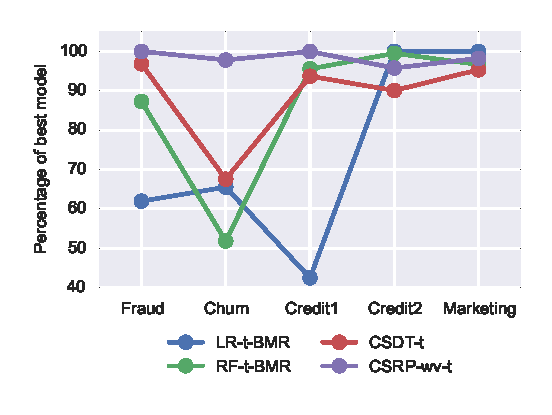
\includegraphics{ch9_fig3}
    \caption{\textbf{Comparison of the savings of the algorithms versus the highest savings in 
    each database.} The $CSRP-wt$ is very close to the best result in all the databases. 
    Additionally, even though the $LR-BMR$ is the best algorithm in two databases, the performance 
    in the other three is very poor.}
    \label{fig:9:comparison_best}
  \end{figure} 
  
  Subsequently, in order to statistically sort the classifiers we computed the Friedman ranking 
  (F-Rank)  statistic \citep{Demsar2006}. This rank increases with the cost of the algorithms. 
  We also calculate the average savings of each algorithm compared with the highest savings in 
each set (perBest), as a  measure of how close are the savings of an algorithm to the best result. 
  In \tablename{~\ref{tab:9:results_ranking}}, the results are shown. It is observed that  the 
  first six algorithms, according to the F-Rank, belong to the $ECSDT$ family. In particular, the 
  best three classifiers is the ensemble of cost-sensitive decision trees using the random patches 
  approach. Giving the best result the one that blends the base classifiers using weighted voting 
  method. Moreover as shown in  \tablename{~\ref{tab:9:results_best}}, this method ranks on each 
  dataset \nth{1}, \nth{2}, \nth{2}, \nth{5} and \nth{3}, respectively. For comparison the best 
  method from an other family is the $RF$ with $BMR$, which ranks \nth{14}, \nth{14}, \nth{8}, 
  \nth{2} and \nth{9}.
   
\begin{figure}[!t]
  \centering
  \subfloat[Comparison of the Friedman ranking.]{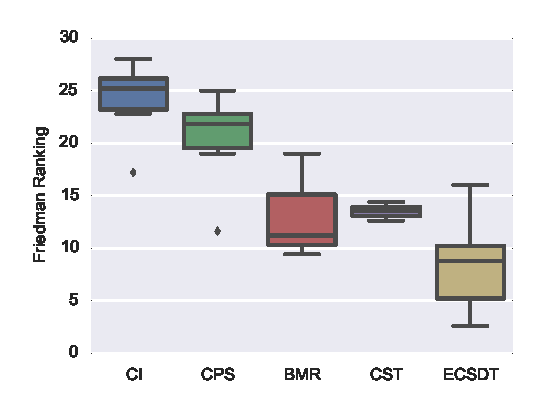
\includegraphics{ch9_fig4}%
    \label{fig:9:family_rank}}
  \hfil
  \subfloat[Comparison of the average savings of the algorithms versus the 
    highest savings.]{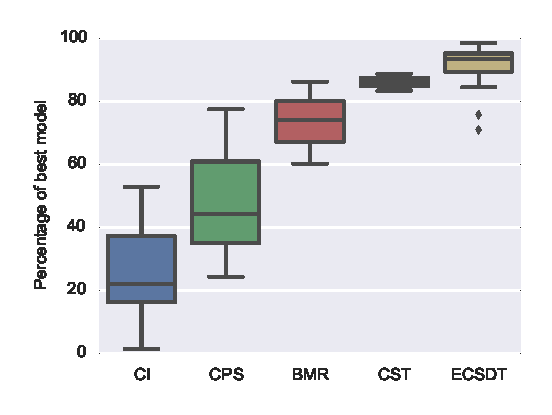
\includegraphics{ch9_fig5}%
    \label{fig:9:family_avgsav}}
  \caption{\textbf{Comparison of the results by family of classifiers.} The $ECSDT$ family has the 
  best performance measured either by Friedman ranking or average percentage of best model.}
  \label{fig:9:comparison_family}
\end{figure}

  Moreover, when analyzing the perBest statistic, it is observed that it follows almost the same 
  order as the F-Rank. Notwithstanding, there are cases in which algorithms ranks are different in 
  the two statistics, for example the $CSDT-t$ algorithm has a lower F-Rank than the $RF-BMR$, 
  but the perBest if better. This happens because, the F-Rank does not take into account the 
  difference in savings within algorithms. This can be further investigated in \figurename{ 
  \ref{fig:9:comparison_best}}. Even that ranks of the $BMR$ models are better than the $CSDT$, the 
  latter is on average closer to the best performance method in each set. Moreover, it is confirmed 
  that the $CSRP-wt$ is very close to the best result in all cases. Lastly, it is shown why the 
  F-Rank of the $LR-BMR$ is high, given the fact that is the best model in two databases. The 
  reason  for that, is because the performance on the other sets is very poor.

   \begin{figure}[!t]
  \centering
  \subfloat[Comparison by inducer methodology.]{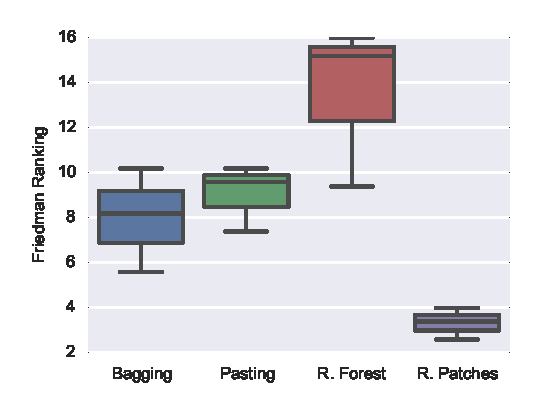
\includegraphics{ch9_fig6}%
    \label{fig:9:rank_ecsdt1}}
  \hfil
  \subfloat[Comparison by combination of base classifiers approach.]{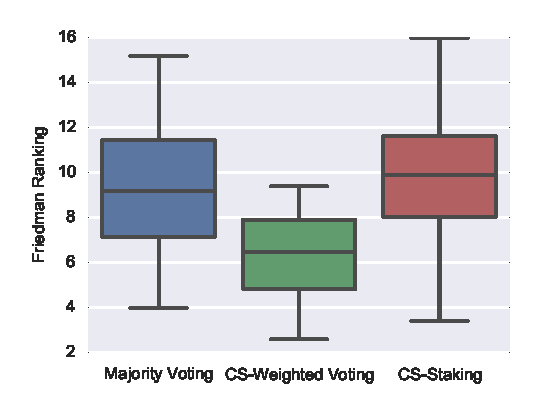
\includegraphics{ch9_fig7}%
    \label{fig:9:rank_ecsdt2}}
  \caption{\textbf{Comparison of the Friedman ranking within the $ECSDT$ family.} Overall, the 
  random inducer method that provides the best results is the $CSRP$. Moreover, the best 
  combination method compared by Friedman ranking is the cost-sensitive weighted voting.}
  \label{fig:9:rank_ecsdt}
\end{figure}

  Furthermore \figurename{~\ref{fig:9:family_rank}}, shows the Friedman ranking of each family of 
  classifiers. The $ECSDT$ methods are overall better, followed by the $BMR$ and the $CST$ methods. 
  As expected, the $CI$ family is the one that performs the worst. Nevertheless, there is 
  a significant variance within the ranks in the $ECSDT$ family, as the best one has a Friedman 
  ranking of 2.6 and the worst 16. Similar results are found when observing the perBest shown in 
  \figurename{~\ref{fig:9:family_avgsav}}. However, in the case of the perBest, the $CST$ methods 
  perform better than the $BMR$. It is important, in both cases it is confirmed that the $ECSDT$ 
  family of methods is the one that arise to the best results as measured by savings.
  
  \begin{figure}[t!]
  \centering
  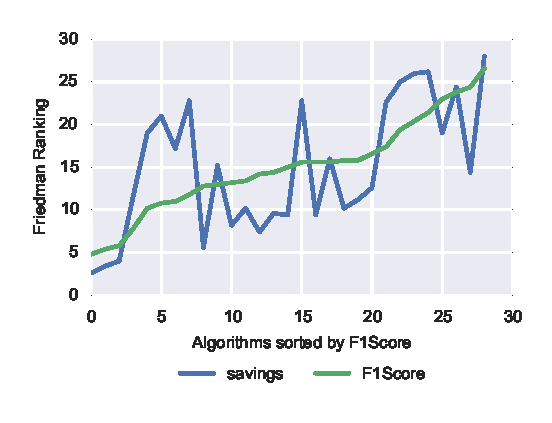
\includegraphics{ch9_fig8}
  \caption{\textbf{Comparison of the Friedman ranking of the savings and F1Score sorted by F1Score 
  ranking.} The best two algorithms according to their Friedman rank of F1Score are indeed the 
  best ones measured by the Friedman rank of the savings. However, this relation does not 
  consistently hold for the other algorithms as the correlation between the rankings is just 
  65.10\%.}
  \label{fig:9:friedman_vs_fscore}
  \end{figure}
  
  We further investigate the different methods that compose the $ECSDT$ family, first by inducer 
  methods and by the combination approach. In \figurename{ \ref{fig:9:rank_ecsdt1}}, the Friedman 
  ranking of the $ECSDT$ methods grouped by inducer algorithm are shown. It is observed that the 
  worst method is the random forest methodology. This may be related to the fact that within the 
  random inducer methods, this is the only one that also modified the learner algorithm in the 
  sense that it randomly select features for each step during the decision tree growing. Moreover, 
  as expected the bagging and pasting methods perform quite similar, after all the only difference 
  is that in bagging the sampling is done with replacement, while it is not the case in pasting. 
  In  general the best methodology is random patches. Additionally, in \figurename{ 
  \ref{fig:9:rank_ecsdt2}}, a similar analysis is made taking into account the combination of base 
  classifiers approach. In this case, the best combination method is weighted voting, while 
  majority voting and staking have a similar performance.

\begin{table}[!t]
     \centering
    \footnotesize
    \begin{tabular}{l l r@{\hskip 0in}c@{\hskip 0in}l r@{\hskip 0in}c@{\hskip 0in}l r@{\hskip 
0in}c@{\hskip 0in}l} %sum 7.7
      \hline
    \bf{Family} & \bf{Algorithm} & \multicolumn{3}{c}{\bf{Fraud}} & 
\multicolumn{3}{c}{\bf{Churn}} & \multicolumn{3}{c}{\bf{Credit 1}} \\
      \hline
CI&DT-t & 0.4458 &$\pm$& 0.0133 & 0.0733 &$\pm$& 0.0198 & 0.2593 &$\pm$& 0.0068 \\
&LR-t & 0.1531 &$\pm$& 0.0045 & 0.0000 &$\pm$& 0.0000 & 0.0494 &$\pm$& 0.0277 \\
&RF-t & 0.2061 &$\pm$& 0.0041 & 0.0249 &$\pm$& 0.0146 & 0.2668 &$\pm$& 0.0085 \\
&DT-u & 0.1502 &$\pm$& 0.0066 & 0.1175 &$\pm$& 0.0103 & 0.2276 &$\pm$& 0.0044 \\
&LR-u & 0.0241 &$\pm$& 0.0163 & 0.1222 &$\pm$& 0.0098 & 0.3160 &$\pm$& 0.0314 \\
&RF-u & 0.0359 &$\pm$& 0.0065 & 0.1346 &$\pm$& 0.0112 & 0.3193 &$\pm$& 0.0053 \\
\hline 
CPS&DT-r & 0.4321 &$\pm$& 0.0086 & 0.1206 &$\pm$& 0.0132 & 0.2310 &$\pm$& 0.0049 \\
&LR-r & 0.1846 &$\pm$& 0.0123 & 0.1258 &$\pm$& 0.0111 & 0.3597 &$\pm$& 0.0156 \\
&RF-r & 0.2171 &$\pm$& 0.0100 & 0.1450 &$\pm$& 0.0131 & 0.3361 &$\pm$& 0.0067 \\
&DT-o & \bf{0.4495} &\bf{$\pm$}& \bf{0.0063} & 0.1022 &$\pm$& 0.0180 & 0.2459 &$\pm$& 0.0081 \\
&LR-o & 0.1776 &$\pm$& 0.0117 & 0.1085 &$\pm$& 0.0203 & 0.3769 &$\pm$& 0.0067 \\
&RF-o & 0.2129 &$\pm$& 0.0080 & 0.0841 &$\pm$& 0.0201 & 0.3281 &$\pm$& 0.0078 \\
\hline 
BMR&DT-t-BMR & 0.2139 &$\pm$& 0.0215 & 0.0941 &$\pm$& 0.0157 & 0.1514 &$\pm$& 0.0390 \\
&LR-t-BMR & 0.1384 &$\pm$& 0.0044 & 0.1370 &$\pm$& 0.0150 & 0.1915 &$\pm$& 0.0340 \\
&RF-t-BMR & 0.2052 &$\pm$& 0.0183 & 0.1264 &$\pm$& 0.0156 & 0.3186 &$\pm$& 0.0072\\
\hline 
CST&CSLR-t & 0.2031 &$\pm$& 0.0065 & 0.1134 &$\pm$& 0.0151 & 0.1454 &$\pm$& 0.0517 \\
&CSDT-t & 0.2522 &$\pm$& 0.0980 & 0.1288 &$\pm$& 0.0194 & 0.2754 &$\pm$& 0.0059 \\
\hline 
ECSDT&CSB-mv-t & 0.2112 &$\pm$& 0.0125 & 0.1481 &$\pm$& 0.0122 & 0.2927 &$\pm$& 0.0108 \\
&CSB-wv-t & 0.2112 &$\pm$& 0.0091 & 0.1686 &$\pm$& 0.0125 & 0.2926 &$\pm$& 0.0108 \\
&CSB-s-t & 0.2072 &$\pm$& 0.0103 & 0.1554 &$\pm$& 0.0121 & 0.2818 &$\pm$& 0.0075 \\
&CSP-mv-t & 0.2098 &$\pm$& 0.0126 & 0.1480 &$\pm$& 0.0136 & 0.2903 &$\pm$& 0.0108 \\
&CSP-wv-t & 0.2099 &$\pm$& 0.0054 & 0.1651 &$\pm$& 0.0120 & 0.2905 &$\pm$& 0.0110 \\
&CSP-s-t & 0.2064 &$\pm$& 0.0069 & 0.1590 &$\pm$& 0.0099 & 0.2809 &$\pm$& 0.0062 \\
&CSRF-mv-t & 0.2208 &$\pm$& 0.0022 & 0.1081 &$\pm$& 0.0224 & 0.2994 &$\pm$& 0.0226 \\
&CSRF-wv-t & 0.2175 &$\pm$& 0.0019 & 0.1220 &$\pm$& 0.0234 & 0.2992 &$\pm$& 0.0236 \\
&CSRF-s-t & 0.2169 &$\pm$& 0.0045 & 0.1304 &$\pm$& 0.0162 & 0.2916 &$\pm$& 0.0236 \\
&CSRP-mv-t & 0.2691 &$\pm$& 0.0054 & 0.1511 &$\pm$& 0.0110 & 0.4031 &$\pm$& 0.0079 \\
&CSRP-wv-t & 0.2780 &$\pm$& 0.0041 & \bf{0.1710} &\bf{$\pm$}& \bf{0.0140} & \bf{0.4049} 
&\bf{$\pm$}& \bf{0.0066}\\
&CSRP-s-t & 0.2735 &$\pm$& 0.0148 & 0.1622 &$\pm$& 0.0103 & 0.3953 &$\pm$& 0.0141 \\
      \hline
      \multicolumn{11}{c}{(those models with the highest F1Score are market as bold)}
    \end{tabular}
\caption{Results as measured by F1Score}
\label{tab:9:results_f1score}
  \end{table}

\begin{table}[!t]
     \centering
    \footnotesize
    \begin{tabular}{l l r@{\hskip 0in}c@{\hskip 0in}l r@{\hskip 0in}c@{\hskip 0in}l  } %sum 7.7
    \hline
    \bf{Family} & \bf{Algorithm} &  \multicolumn{3}{c}{\bf{Credit 2}} 
& \multicolumn{3}{c}{\bf{Marketing}} \\ 
      \hline
CI&DT-t &  0.2614 &$\pm$& 0.0083 & 0.2647 &$\pm$& 0.0079\\ 
&LR-t & 0.0155 &$\pm$& 0.0037 & 0.2702 &$\pm$& 0.0125\\ 
&RF-t &  0.0887 &$\pm$&0.0061 & 0.2884 &$\pm$& 0.0116\\ 
&DT-u &  0.3235 &$\pm$&0.0055 & 0.2659 &$\pm$& 0.0061\\ 
&LR-u &  \bf{0.3890} &\bf{$\pm$}& \bf{0.0053} & 0.3440 &$\pm$& 0.0083\\ 
&RF-u & 0.3815 &$\pm$&0.0051 & 0.3088 &$\pm$& 0.0065\\ 
\hline 
CPS&DT-r &0.3409 &$\pm$&0.0046 & 0.2739 &$\pm$& 0.0076\\ 
&LR-r &  0.3793 &$\pm$& 0.0049 & 0.3374 &$\pm$& 0.0101\\ 
&RF-r & 0.3570 &$\pm$& 0.0048 & 0.3103 &$\pm$& 0.0075\\ 
&DT-o & 0.3258 &$\pm$& 0.0056 & 0.2634 &$\pm$& 0.0089\\ 
&LR-o & 0.3804 &$\pm$& 0.0044 & \bf{0.3568} &\bf{$\pm$}& \bf{0.0102}\\ 
&RF-o & 0.3212 &$\pm$& 0.0054 & 0.3083 &$\pm$& 0.0093\\ 
\hline 
BMR&DT-t-BMR & 0.3338 &$\pm$& 0.0052 & 0.2433 &$\pm$& 0.0071\\ 
&LR-t-BMR &  0.3572 &$\pm$&0.0045 & 0.2954 &$\pm$& 0.0079\\ 
&RF-t-BMR &  0.3551 &$\pm$&0.0053 & 0.2744 &$\pm$& 0.0070\\ 
\hline 
CST&CSLR-t & 0.3363 &$\pm$&0.0045 & 0.2339 &$\pm$& 0.0051\\ 
&CSDT-t & 0.3483 &$\pm$& 0.0046 & 0.2680 &$\pm$& 0.0060\\ 
\hline 
ECSDT&CSB-mv-t & 0.3503 &$\pm$& 0.0046 & 0.2758 &$\pm$& 0.0072\\ 
&CSB-wv-t &  0.3503 &$\pm$&0.0046 & 0.2757 &$\pm$& 0.0072\\ 
&CSB-s-t &  0.3533 &$\pm$& 0.0046 & 0.2799 &$\pm$& 0.0074\\ 
&CSP-mv-t &0.3499 &$\pm$& 0.0044 & 0.2749 &$\pm$& 0.0064\\ 
&CSP-wv-t & 0.3498 &$\pm$&0.0045 & 0.2749 &$\pm$& 0.0064\\ 
&CSP-s-t &  0.3524 &$\pm$&0.0046 & 0.2778 &$\pm$& 0.0104\\ 
&CSRF-mv-t & 0.3560 &$\pm$&0.0118 & 0.2780 &$\pm$& 0.0106\\ 
&CSRF-wv-t & 0.3549 &$\pm$&0.0069 & 0.2552 &$\pm$& 0.0187\\ 
&CSRF-s-t &  0.3540 &$\pm$&0.0071 & 0.2578 &$\pm$& 0.0186\\ 
&CSRP-mv-t &0.3743 &$\pm$& 0.0050 & 0.2916 &$\pm$& 0.0062\\ 
&CSRP-wv-t & 0.3721 &$\pm$& 0.0051 & 0.2781 &$\pm$& 0.0063\\ 
&CSRP-s-t & 0.3720 &$\pm$& 0.0049 & 0.2922 &$\pm$& 0.0137\\ 
      \hline
      \multicolumn{8}{c}{(those models with the highest F1Score are market as bold)}
    \end{tabular}
\caption{Continuation of \tablename{~\ref{tab:9:results_f1score}}}
\label{tab:9:results_f1score2}
  \end{table}

  Finally, in \tablename{~\ref{tab:9:results_f1score}} the results of the algorithms measured by 
  F1Score are shown. It is observed that the model with the highest savings is not the same as the 
  one with the highest F1Score in all of the databases, corroborating the conclusions from 
  \citep{CorreaBahnsen2013}, as selecting a method by a traditional statistic does not give the 
  same result as selecting it using a business oriented measure such as financial savings. This can 
  be  further examined in \mbox{\figurename{~\ref{fig:9:friedman_vs_fscore}}}, where the ranking of 
  the F1Score and savings are compared. It is observed that the best two algorithms according to 
  their Friedman rank of F1Score are indeed the best ones measured by the Friedman rank of the 
  savings. However, this relation does not consistently hold for the other algorithms as the 
  correlation between the rankings is just 65.10\%. 
